\section{Ændringer af testdesign}
\label{TestAfSkalaerAendringerTD}
%
Efter at have afviklet testen i AAL den 01-12-2017 var der indsamlet data fra 22 testpersoner. Da det tilstræbes at have omkring 45 testpersoner blev det derfor besluttet at tage ud i lufthavnen og indsamle mere data den 05-12-2017. Information om afgangene blev derfor opdateret, så de passede til den tilsvarende dag testen blev kørt. 

Ydermere blev det under testen observeret, at det var svært at styre hvor tæt på og fra hvilken vinkel robotten henvendte sig. Selvom det blev prøvet at følge skemaet, var der mange rejsende, som undveg robotten, når den kom for tæt på eller generelt ikke virkede til at have lyst til at interagere med den. Det blev derfor besluttet at prøve at variere de forskellige typer henvendelser, men uden at følge et bestemt skema. Da de rejsende også generelt virkede til at være mindre interesserede i robotten på de to testdage sammenlignet med de rejsende i feltundersøgelsen, blev det besluttet at det var vigtigere at få nogle testpersoner frem for at følge et bestemt skema. Højden på robotten blev i starten varieret efter skemaet, men som der blev mangel på testpersoner blev det besluttet at variere højden oftere, så alle højder blev testet.

I lufthavnen var der en testperson, som gerne ville vide hvor toilettet var, men ikke ville følges derhen. Vedkommende virkede lidt forvirret da robotten efterfølgende spurgte hvad den så kunne hjælpe med, hvorefter vedkommende gik. Det valgtes derfor, at hvis der trykkes nej til gældende spørgsmål, så skifter skærmbilledet til: "Hav en god rejse" og robotten spørger derfor ikke hvad den skal hjælpe med endnu en gang.

\section{Testpersoner}
\label{ParametreFaktiskeTestpersoner}
%
Der er i alt 43 testpersoner, som har interageret med robotten for derefter at svare på de forskellige skalaer. Testpersonerne udgør 16 kvinder og 27 mænd i et aldersspænd fra 10 til 72 år, (M=40.1, SD=13.4). En enkel testperson, TP2, nåede ikke at udfylde sin alder, hvorfor alderen er estimeret til at være 40 år. Observationer gjort for de enkelte testpersoner er beskrevet i \fullref{TestAfSkalaLufthavnsBesog}. Testpersonerne rejser mellem 1 og 100 gange om året (M=15.3, SD=18.1). Dette er udregnet efter testpersonernes nedskrevede besvarelser, hvor nogle testpersoner har svaret et interval, eksempelvis 1-2 gange om måneden eller 6-8 gange om året. Ved svar som 1-2 gange om måneden er det omregnet til antal gange om året, hvorefter det midterste tal er medtaget. Ved svar som 6-8 gange om året er det medtaget at testpersonen rejser 7 gange om året. Hvis testpersonen eksempelvis har svaret 2-3 gange om året er det højeste antal rejser medtaget.
%
\begin{figure}[H]
\centering
\begin{minipage}{.5\textwidth}
  \centering
  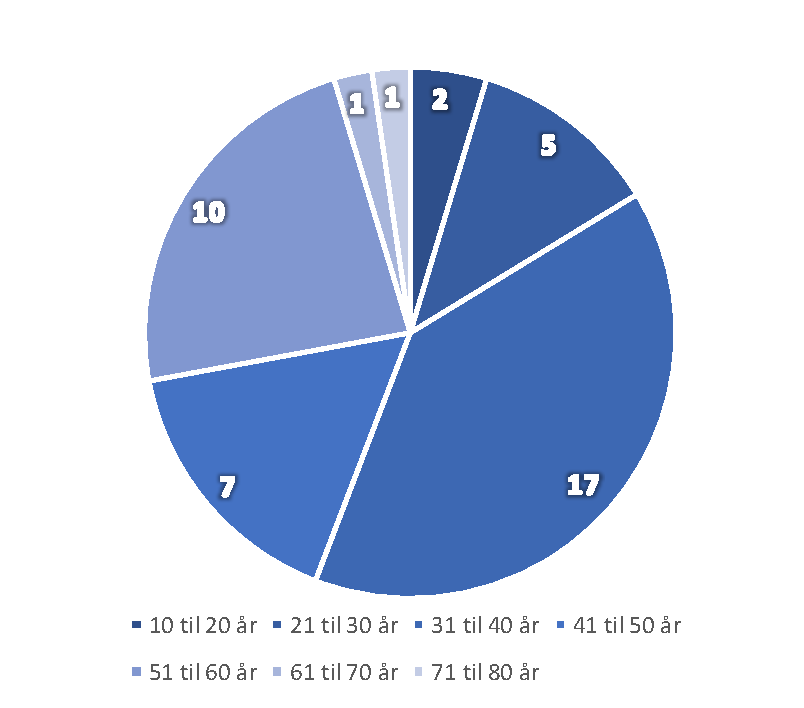
\includegraphics[width=\linewidth]{Figure/DatabehandlingSkalaer/DataPresentation/CirkelDiagramAlder}
  \caption{Testpersonernes aldersfordeling, angivet i antal.}
  \label{fig:CirkelDiagramAlder}
\end{minipage}%
\begin{minipage}{.5\textwidth}
  \centering
  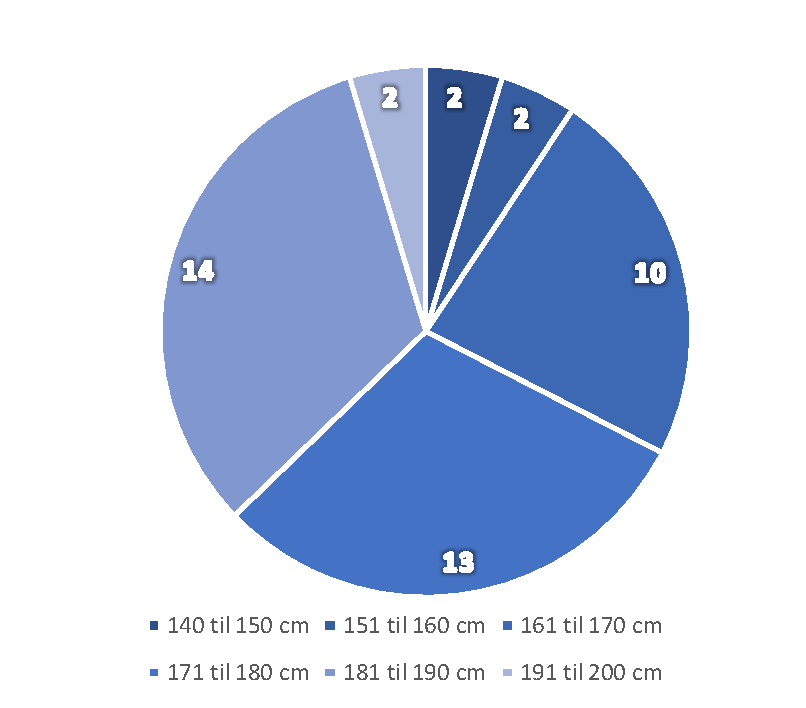
\includegraphics[width=\linewidth]{Figure/DatabehandlingSkalaer/DataPresentation/CirkelDiagramHoejde}
  \caption{Testpersonernes højdefordeling, angivet i antal.}
  \label{fig:CirkelDiagramHoejde}
\end{minipage}
\end{figure}
\noindent
%
Aldersfordelingen fremgår af \autoref{fig:CirkelDiagramAlder}, hvor det fremgår at størstedelen af testpersonerne har været mellem 31 år og 40 år, efterfulgt af 51 år til 60 år, med henholdvist 17 og 10 testpersoner i hver aldersgruppe. Højdefordelingen fremgår af \autoref{fig:CirkelDiagramHoejde}, hvor det fremgår, at størstedelen af testpersonernes højde er mellem 161 cm til 190 cm. Mændende havde en gennemsnitshøjde på 182.1 cm (SD=6.1) og kvinderne havde en gennemsnitshøjde på 164.9 cm (SD=10.8). 